\documentclass[runningheads]{llncs}

\RequirePackage[
  % backend=bibtex,   % Recommended is `biber`, but gives
  backend=biber,     % timeout on Overleaf
  style=numeric,   % Equivalent to elsarticle-num-names
  sorting=none,    % Adjust sorting as needed
  natbib=true      % Compatibility with natbib
]{biblatex}

\usepackage{graphicx}
% \usepackage{cite} % Incompatible with biblatex
\usepackage{url}
\usepackage{lipsum}                     % Dummytext
\usepackage{xargs}                      % Use more than one optional parameter in a new commands
\usepackage[pdftex,dvipsnames]{xcolor}  % Coloured text etc.
\usepackage{subcaption}


% Define custom colors
\definecolor{irrelevant}{RGB}{255, 0, 0} % Red color for old text
\definecolor{old}{RGB}{128, 128, 128} % Gray color for irrelevant text
\definecolor{final}{RGB}{0, 128, 0} % Green color for final text
\definecolor{edit}{RGB}{0, 0, 255} % Blue color for notes or other text


% Increase margin text width
\setlength{\marginparwidth}{2cm}

\usepackage{scrlayer-scrpage}

% Bibliography:
\addbibresource{bibliography/phd_proposal.bib}
\addbibresource{bibliography/lit_review_specific.bib}
\addbibresource{bibliography/zoom_calib.bib}

\setcounter{page}{1}

%
% ============== Define custom TODO commands ===========================
\usepackage[
  colorinlistoftodos,
  prependcaption,
  textsize=tiny,
  % disable
  ]{todonotes}

\newcommand{\comment}[2][Comment]{\todo[inline,color=blue!20!white]{\textbf{#1}: #2}}
\newcommand{\commentside}[2][Comment]{\todo[color=blue!20!white]{\textbf{#1}: #2}}
\newcommand{\fixme}[1]{%
  \todo[color=red!20, inline, size=\footnotesize]{FIXME: #1}%
}
\newcommand{\review}[1]{%
  \todo[color=blue!10, inline, size=\footnotesize]{REVIEW: #1}%
}

% With an exclamation mark icon
\newcommand{\alert}[1]{%
  \todo[inline, color=orange!30, size=\small, bordercolor=orange!80, linecolor=orange!80]{ALERT: #1}%
}

% ============== END: Define custom TODO commands ===========================

\makeatletter
\AtBeginDocument{%
  \def\doi#1{\url{https://doi.org/#1}}}
\makeatother

\makeatletter
\renewcommand\paragraph{\@startsection{paragraph}{4}{\z@}%
                                    {2.25ex \@plus1ex \@minus.2ex}%
                                    {-1em}%
                                    {\normalfont\normalsize\bfseries}}
\makeatother

% ============ BEGIN ToC Style ============

% Define the ToC style:
% - skip the document title itself in the ToC
% - include sections and subsections in ToC
\makeatletter
% Keep a copy of LNCS’s original \maketitle
\let\origlncsMaketitle\maketitle

\renewcommand{\maketitle}{%
  \begingroup
    % Disable \addcontentsline while the title is created
    \let\savedaddcontentsline\addcontentsline
    \renewcommand{\addcontentsline}[3]{}
    % Call LNCS's original macro
    \origlncsMaketitle
  \endgroup
}
\makeatother
\setcounter{tocdepth}{3} % Includes sections and subsections

% ============ END ToC Style ===============


\begin{document}

\sloppy % to avoid text going out of margins, compilation errors on formatting in development phase.

%
\title{
  UGV Long Range Backtracking Recovery in Unstructured Outdoors Environment Using Active Visual Landmarks Navigation:
  Literature Review
}

\author{Dmytro Kushnir\orcidID{0009-0006-8652-5781} }
%
\authorrunning{D. Kushnir}
% First names are abbreviated in the running head.
% If there are more than two authors, 'et al.' is used.
%
\institute{
  Ukrainian Catholic University, L'viv, Sventsitskogo st. 17,  79011, Ukraine
  \email{kushnir\_d@ucu.edu.ua}
}
%
\maketitle              % typeset the header of the contribution
%

\tableofcontents


\section{Introduction}

\subsection{Motivation}

The advancement of autonomous systems in industries such as agriculture, mining, and military technology is hindered by the lack of open-source tools. These sectors demand robust, adaptable technologies to operate in unstructured environments. Addressing these challenges is crucial not only for technological progress but also for democratizing access to innovations.

\todo{Briefly expand on how open-source tools like ROS have driven innovation and how they can address current limitations.}

\subsection{Problem Statement}

\textbf{Problem Statement:} Unstructured environments, characterized by the absence of predefined landmarks and inconsistent terrain, present unique challenges for autonomous navigation. These challenges necessitate systems capable of robust perception, reasoning, and adaptability.

\todo{Clarify the specific characteristics of unstructured environments and their implications for long-range navigation and backtracking.}

\subsection{Methodology of Review}

This work adopts a structured approach to literature review, guided by design-driven analysis. The  "System Design Loop (Task-Requirement-Design-Validation)" framework serves as the foundation for selecting and evaluating relevant studies. Focus areas include:
\begin{itemize}
    \item Systematic reviews and large-scale almanacs covering robotics research.
    \item DARPA-like challenge-driven studies that benchmark real-world performance.
    \item High-impact papers with implementations adaptable to ground robotics.
\end{itemize}
\todo{Detail the search and filtering process for the literature review. Mention tools like citation analysis or database usage.}

\subsection{Structure of the Review}

The review is organized as follows:
\begin{itemize}
    \item Traits of robotics research literature, highlighting key patterns and challenges.
    \item Design-guided analysis, presenting problem decomposition and solution strategies.
    \item Review of primary goals and research gaps, including secondary constraints.
    \item Conclusions and future directions for iterative analyze-design-implementaion cycles, modular and open-source solutions.
\end{itemize}
\comment[]{Add references to relevant sections and refine the flow as needed.}

\section{Bibliometric Traits of Robotics Research Literature}

\comment[]{ This section highlights findings, hypotheses, and key observations in robotics literature, aiming to guide literature review methodology and explain its context to non-specialists. }

\subsection{Factors in Robotics Domain}
Research in unstructured UGV robotics specifically impacted by next factors, which are not typical for other robotics domains:

 \paragraph{Large-scale reviews or almanacs}
  (aggregating 250+ papers) play a critical role in providing comprehensive overviews of the field. Here we will write a bit and try to understand the reasons behind the unusual number and high quality of the large-scale reviews and almanacs in robotics research.
  \todo{Add more details and references to existing researches from the bibliography.}

\paragraph{The Volume of publications} is significantly smaller than in mainstream AI, where research output is orders of magnitude higher.

Unlike mainstream AI, which experiences terminological saturation, robotics remains more fragmented. For instance, the seminal robotics paper "FastSLAM: A factored solution to the simultaneous localization and mapping problem" (2002) has accrued approximately 3,500 citations in 20 years. In contrast, the AI paper "BERT: Pre-training of Deep Bidirectional Transformers for Language Understanding" (2018) achieved 50,000 citations in just five years. \todo{Add reference to resources with citation statistics.}

These differences show that citation-based snowballing approaches are less effective for navigating robotics literature. Instead, classic analysis of comprehensive reviews, challenge-driven studies, and large-scale almanacs are better suited to understanding the field.

\paragraph{Man-made Challenge-Driven Clusters}
 Research initiatives, such as DARPA and MBZIRC challenges, drive progress by clustering studies around specific problems.

   There are expected "clusters" or "clogs" in the robotics research publications. Not only around the dedicated fields, problems, and laboratories which occur in a natural way in each field of research.
  The non-typical thing is research streamlined by strategic governmental organizations. The most well-known is DARPA. Now there are more of them, like MBZIRC.

 \todo{Add something later, support with citations.}

  \paragraph{Industry-lead Researches}
  The research kits of new devices are widely distributed specifically amongst the researchers and other contributors to the public domain.
  Similar clusters are streamed by non-governmental organizations: technical giants.
  \todo{describe the case of Kinect. Examples by Intel, OpenCV, Cameras series... }

  \paragraph{Long-term stationary groups.} Research is typically long-term and conducted by well-established teams with access to substantial resources.

  \paragraph{Poor comparison ground.} The field lacks standardized benchmarks or datasets, making cross-comparisons between studies challenging.

  What matters most in this field is the careful formulation of problems and the requirements they impose. These requirements drive the system design of solutions, followed by implementation and validation. Unlike AI, where isolated benchmarks play a central role, robotics focuses on real-world conditions, versatility, robustness, and iterative improvements.

  Robotics research is often fragments across variables such as indoor versus outdoor environments, aerial versus ground platforms, and real-time versus non-real-time systems. Addressing these distinctions narrows the scope of each research problem, creating a "pin-tip" scale for the research frontier. With a smaller research community, large-scale benchmarks or datasets are often absent.

  This fragmentation explains why research frequently focuses on specific, everyday tasks that extend beyond current robotics capabilities. One example is the "returning home" problem, a fundamental yet challenging task. Relevant papers on such tasks tend to cluster around research centers, datasets, or individual experts.

\subsection{Public and Private SOTA}
  Public SOTA contrasts with proprietary solutions, revealing a reproducibility crisis in robotics academia caused by platform-locked tools. Proprietary systems hinder progress, while public SOTA relies on open platforms, albeit with limitations in scalability and resources.
  \todo{Explore the coined term "Public SOTA" and its broader implications.}

\subsection{Citations Connectivity Pattern in Robotics Research}

\comment[]{The abpvementioned traits and arguments are leading to this one. Here we illustrate by example this connectivity.}

\begin{figure}[ht]
  \centering
  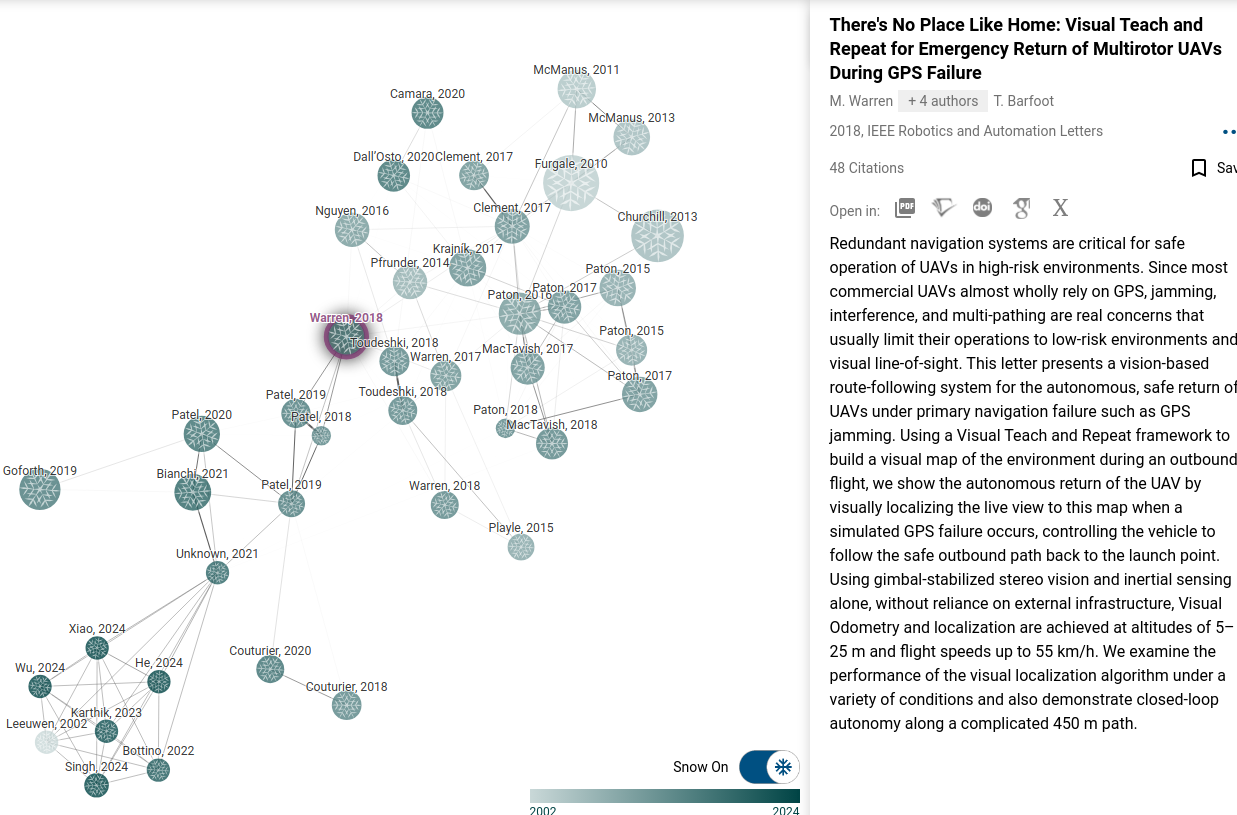
\includegraphics[width=\linewidth]{img/There_is_no_place_like_home_research_tree.png}
  \caption{Visual Teach-and-Repeat approach for emergency return of multirotor UAVs during GPS failure \protect\cite{warren-ral19-no-place-like-Home}. More information is available on Connected Papers: \protect\url{https://www.connectedpapers.com/}.}
  \label{fig:no_place_like_home}
\end{figure}

The papers in this field are well connected, and the research is often conducted within "clusters" of research groups. An example of such clustering can be seen in the work of Warren et al. (Figure~\ref{fig:no_place_like_home}), which demonstrates the modest size but tight connections of research within this domain.

\todo{Amplify with examples of explosive technology disruptions, e.g., Kinect or ROS2.}

\subsection{Other Traits}

\comment[Here we will accumulate smaller findings and hypothesis that are not explained. Those can enhanced the main ones, are derrived from them, etc.]{}

\begin{itemize}
  \item Academia is tied to the industrial RnD. The researchers have to use the same equipment for repeatability of results and ecosystem support.
  \item Industry-lead researches: research kits of new devices are widely distributed specifically amongst the researchers and other contributors to the public domain.
  \item Public domain stearing largely by the Private entities.
  \item Different equipment on research and mature application stages.
  \item Governemntal interests and policies involved in stearing the research programs. (More then in other fields.)
\end{itemize}

All listed above helps us to better understand, why the part of community that remain independent are so uncompromising on their rules and policies to reensure it.

\comment[]{Here we are talking about unusual level of self-conscious and organization in Academy+PublicDomainCommunity in the field of robotics. ROS is one of those strategic project organized and nurished by them (companies as WillowGarage and etc.)}



\section{Design-Guided Literature Review}

\comment[]{
  At first about methodology of review that we propose.
  Then we do the analysis of the problem and requirements.
  Here we will meticulously deconstruct the whole challenge into a set of requirements, investigate the available set of approaches, tradeoffs, and design the solution aspects. The CORE of literature analysis in robotics will be here. In such a manner we will ensure that we are solving the actual large-scale problem applicable beyond our setup.
}

Additional factors that guided the literature review process include:
\begin{itemize}
  \item Preference was given to studies with implementations adaptable to our platform or those offering detailed ground truth data demonstrations.
  \item Industry standards and widely adopted tools, especially those with robust GitHub repositories, community, and version updates were emphasized to ensure practical relevance and reproducibility.
\end{itemize}

\subsection{Analysis Framework}

\comment[At first subsection we describe the analysis framework. In upcomming sections we use it and comment our findings.]{}

The review leverages a structured "Task-Requirement-Design-Implementation-Validation" methodology.

\todo{Find sources that describe this methodology of design and research.}

\textbf{
 Steps fo that we do:
}
- Task: Select the problem we are dealing with: from the needs to the vision of the solution.
- Requirement: Decompose task into some basic tasks, stages, states. Constraints also come here as the type of requirements. Decompose single iteration at once, maintain a higher level of abstraction.
- Design:
  Here we have to envision the idea of the system that can satisfy those requirements on the highest level. In Robotics, reusability is the key, so here we have to narrow the application domain and look for existing solutions.
- Search the literature for the solutions that can satisfy the placed requirements.
- Filter the results.
  - Prioritize the experiments or stages of implementations.
- "Allocate" the requirements to system components.

\todo{Include visual diagrams or reference placeholders for MeROS-based design layers.}

\subsection{Task-Requirement-Design Analysis of the Problem}

Here, when the spefific traits of the research field is mapped and analysis approach is selected, we should understand why this problem is not solved till this moment in selected conditions. Those limitations will be the requirements for the solution.

This will give us a hypothesis that we will work with.

For sure, when we are launching the research in any direction, the surrounding problems are also might be an issue. So beside of core research gaps (our main focus) we will need to pay attention to factors that are making risks for the solution.

Some limitations of given design we should see from the design phase: we incorporate them consciously. They are derived from the whole collection of requirements in the most explicit way -- designed limitations are "the requirements that are not allocated or even mentioned". But the big part of limitations will come up only after the validation stage of research.

Clarifying our goal as well (new ideas and vision of the problem has to rise from the first validation stage), we will map them as unallocated requirements and address them in the next iterations of the work.

The first iteration should include the bare minimum of the requirements. This is the most dangerous part of the project, where we have the most uncertainty.
From the first pilot implementation state, we will be able to map the iterations towards the desired system with all requirements satisfied.

Each iteration of the process will satisfy one or more new requirements.

\todo{Place the example of work phases scheme. Example on how we will get to the PTZ camera is the best candidate.}

\section{Problem Decomposition Outcomes}

\comment[Here we have already decomposed problem, next step is to analyze each subfield separetely. Here we are doing the actual subject-by-subject review of the subfields fields.]{}

\subsection{Primary Goals and Objectives}

\comment[We will concentrate our research efforts on them specifically]{}

\begin{itemize}
  \item Active Visual Navigation: Pan-Tilt-Zoom camera and integration challenges.
  \item Long-range Backtracking in unstructured environments.
        \begin{itemize}
          \item No-map navigation recovery and its limitations.
          \item Representation of places.
          \item Route following between places with minimal memorization.
        \end{itemize}
  \item Encapsulation of system modules: software and hardware requirements.
  \item Cross-platform interfacing requirements.
  \item Calibration and data processing for open-source robotics.
\end{itemize}

\subsubsection{Mapping Approaches}
Summarize current techniques in mapping for unstructured environments.
\todo{Discuss strengths and limitations of existing methods.}

\subsubsection{Active Visual Navigation: Applications of Pan-Tilt-Zoom (PTZ) Camera }

\comment[]{Discuss the role of PTZ cameras in UGV platforms, emphasizing modular design and requirement-based development.
}

\todo[inline]{Include examples of modular designs and calibrations.}
\todo[inline]{Explore alternative solutions tradeoffs, like 360-degree cameras or other configurations.}

\paragraph{PTZ Camera Integration Challenges}

\comment[Calibration and opensource limitations]{ We discover the entry barriers for the PTZ camera integration. The main problem is the lack of open-source calibration tools and the absence of standardized interfaces. We planned and started the research direction with first results. }

\subsection{Constraints and Challenges}
\comment[Here we review the "secondary objectives". Those are factors that can have a decisive impact on the feasibility of the task. Therefore they require our attention, but fell out of the main focus of the research]{}

\subsubsection{Datasets}

A few datasets can serve as a basis for this research or as a sign of missing data:
\begin{itemize}
  \item Wild Scenes Dataset: \url{https://arxiv.org/pdf/2404.18477}
  \item Wild Places Dataset: \url{https://csiro-robotics.github.io/Wild-Places}
  \item Freiburg Forest: \url{https://paperswithcode.com/dataset/freiburg-forest}
\end{itemize}
\todo{Note the gaps in available datasets and propose directions for addressing these limitations.}

\subsubsection{Simmulation Environments}

\comment[]{ For evaluation of the agent's behavior and holistic autonomous system integration we will need the simulation environment. The most popular is Gazebo. But there are other solutions. We will review them and propose the best one for our research.}

\subsubsection{Hardware Limits}
\begin{itemize}
  \item Planning and power management.
        Long-range navigation is limited by the energy capacity of the UGV and the efficiency of its spending.
  \item Environmental factors such as weather, light, and terrain complexity.
        This parameter has to be mentioned, to clearly denote limitations of considered conditions.
  \item Real-time processing requirements.
        The real-time processing of sensor data and decision-making are important for robotics, but we outline the problem and design solution in such a manner to allow for the relaxations on this requirement.
  \item Scalability and integration with ROS platforms.
        As we touch lots of system aspects with limited resources, we will focus on the iterative implementations and open solutions.
\end{itemize}

\todo[inline]{Discuss relaxations on real-time requirements and focus on iterative implementations.}

\subsubsection{The Impact of the ROS-based Solutions}

\comment{This is a Larger piece of text for ROS. Other aspects will be detailed in a similar fashion + add references}

The Robot Operating System (ROS) has emerged as a cornerstone technology in the robotics field, providing an open-source framework that standardizes development and fosters collaboration across academia and industry. Its modular architecture allows researchers and developers to integrate diverse hardware and software components, enabling rapid prototyping and scalability for a wide range of applications.

One of ROS's most significant contributions is its community-driven ecosystem, where shared libraries, tools, and documentation accelerate innovation. ROS supports real-time applications, bridging the gap between laboratory research and field deployment. This feature has proven particularly valuable in unstructured environments, where dynamic conditions demand robust and flexible solutions. Moreover, the adoption of ROS by industry leaders has enhanced its relevance, making it a platform that seamlessly connects academic research with practical deployment.

In the context of this review, ROS plays a pivotal role in the development of modular designs, such as the MeROS framework. By leveraging ROS's tools for sensor integration, motion planning, and communication, MeROS exemplifies how a standardized platform can streamline the design and validation of complex robotic systems. However, despite its strengths, ROS is not without limitations. Challenges such as real-time processing constraints, hardware compatibility, and dependency management persist, leaving room for further enhancements.

\subsection{System Limitations and Implementation Milestones}

\comment[Here we will discuss the Limitations that we've faced during the validation-by-implementation]{}

\section{Conclusion and Further Research Motivation}

\comment{
Overall here I want to say how this particular research is important in the field of UGV autonomy. But itself is just a POC of systematic approach to break the current limitations that are stopping this field of robotics.
We discovered that the field requires methodological instruments to organize the RnD efforts.
 That by iterations and achievement of the final goal of this project we will see if the field are succeptible to ours disruptions and what changes we should add to the methodology before the introducing it to the new schools of researchers.

  - Summarize again the Goals->Pipeline->Particular outcomes.
  - Discuss the potential impact of the research on the field.
  - Highlight the significance of open-source contributions and iterative validation in advancing the field.
  - Discuss the future work and the next steps.
}


The proposed research aims to:
\begin{itemize}
  \item Emphasize modular design and cross-platform usability.
  \item Identify critical bottlenecks halting advancements.
  \item Validate the feasibility of addressing these bottlenecks through:
        \begin{itemize}
          \item Open-source calibration and integration tools.
          \item Testing on Husky UGV or equivalent platforms.
          \item Clear documentation and interfaces following MeROS philosophy.
        \end{itemize}
\end{itemize}

\todo[inline]{Highlight the significance of open-source contributions and iterative validation in advancing the field.}

\subsection{Future Work}

\begin{itemize}

  \item Prepare the proper publication of the results.
  \item Explore different \textbf{ Languages, beside English }, to find the most comprehensive set of the literature.
  \item Develop the system to the level of first prototype. This has to preclude the publication. We need to validate our Design and Literature findings at least on the feasibility level.
  \item In the course of publication preparation also include other tools and approaches to validate some unsipported assumpions and hypothesis about research field structure: systematically use snowballing, citation analysis, and other tools to validate the structure of the field.
  \item Explore adjacent fields.
  \item Do comparison with the other approaches. (Approach was not validated explicitly)
  \item
\end{itemize}


\printbibliography

\end{document}
